\chapter{Metodología}

En este capítulo se describen los procedimientos que se llevaron a cabo a lo largo de este trabajo. El objetivo es presentar el flujo de desarrollo, el cual comienza con la obtención y preparación de los datos (Sección~\ref{sec:obtencion_datos_section}), continúa con la construcción de un \textit{benchmark} con métodos que se han desarrollado previamente para resolver el problema en cuestión (Sección~\ref{sec:Benchmark_section}), la construcción del grafo de Internet (Sección~\ref{sec:creacion_grafo_section}), y finaliza con el diseño de modelos basados en Redes Neuronales de Grafos (Sección~\ref{sec:gnn_section}).\\

A modo de recapitulación, el problema abordado en este trabajo de tesis consiste en la inferencia de los tipos de relaciones económicas que comparten los Sistemas Autónomos (AS) en la red de Internet, por medio del uso de Redes Neuronales de Grafo. Durante todo el desarrollo se utilizó el lenguaje de programación Python y, en particular, se utilizaron las bibliotecas de Pytorch~\cite{Pytorch} y DGL~\cite{DGL} (Deep Graph Library) para la implementación de las GNNs, NetworkX~\cite{networkx} para la creación y manipulación de grafos y las bibliotecas estándar para el manejo de datos y otras funciones de utilidad.\\

El desarrollo del proyecto está organizado en dos repositorios. El primero, dedicado al \textit{benchmark}~\cite{BenchmarkCode}, el cual contiene las implementaciones de métodos preexistentes para la tarea de inferencia de relaciones entre ASes, mientras que el segundo repositorio~\cite{gnnCode} se encuentra enfocado en la construcción de un grafo de Internet y la aplicación de modelos basados en GNNs, además de incluir otros experimentos complementarios realizados durante el estudio.\\

%-----------------------------------------------------------------------------------------------------------------------------------------------------------------------------------------------------

\section{Obtención de Datos} \label{sec:obtencion_datos_section}


\subsection{Fuentes de Datos}
% Importancia de datos y dedonde se saco
La obtención de datos fue una etapa fundamental en el trabajo, comenzando con la búsqueda de fuentes confiables y de acceso público para obtener información sobre la topología de Internet. Para esto, se revisaron trabajos relacionados con el área de redes y el protocolo BGP, estudiando las fuentes de datos utilizadas en dichos estudios. Este proceso permitió identificar los conjuntos de datos utilizados comúnmente, provenientes principalmente de las iniciativas: RIPE RIS~\cite{RIPE-RIS}, RouteViews Project~\cite{RouteViewsProject}, CAIDA~\cite{CAIDA} y PeeringDB~\cite{PeeringDB}.\\

% desaffio
%\subsection{Desafíos de acceso y organización}

\vspace{0.5cm}
Uno de los principales desafíos de esta etapa fue la forma en que los datos se encuentran 
%\seba{en la versión final hay que evitar que queden líneas sueltas al final o al inicio de cada página. mientras estemos en borrador, no nos preocupemos de esto, pero hay que considerarlo finalmente.} 
organizados en sus respectivas plataformas. En general, estas presentan una estructura poco clara, con escasa documentación. Esto dificultó inicialmente la comprensión del contenido y el uso de la información. Sin embargo, a medida que se profundizó en el estudio y se revisaron trabajos previos, fue posible familiarizarse con los datasets utilizados para el análisis y estudio de Internet y el protocolo BGP.\\


% Objetivo de cada una de las plataformas de datasets
La dificultad de comprensión de estas páginas radica principalmente en que muchos estudios e información se repetían de distintas formas. Sin embargo, esto se debe a que cada fuente responde a objetivos distintos. CAIDA~\cite{CAIDA} actúa como repositorio de datos y estudios en el área de redes. RouteViews Project~\cite{RouteViewsProject} (RV), por otro lado, se enfoca en el uso de colectores ubicados en lugares estratégicos de la infraestructura de Internet, ofreciendo así datos BGP ``crudos'' (RIBs y mensajes \textit{UPDATE}) útiles para reconstruir el estado de enrutamiento en instantes específicos. Por último, RIPE RIS~\cite{RIPE-RIS} también mantiene una red de recolectores, pero además ofrece otros proyectos de medición del Internet así como servicios en tiempo real y \textit{datasets} complementarios.
Más información específica sobre las fuentes de datos puede encontrarse en el Anexo~\ref{sec:anexo_recoleccion_datos_internet}.\\

Finalmente, es importante destacar que estas fuentes proporcionan una visión parcial de la topología de Internet. En particular, los datos BGP observados desde RouteViews y RIPE RIS dependen de la cantidad y ubicación de los colectores y \textit{vantage points} disponibles, por lo que no todos los enlaces existentes en la red quedan necesariamente reflejados en las rutas recolectadas. Esta limitación es especialmente relevante en el caso de enlaces \textit{peer-to-peer} y conexiones privadas, cuya visibilidad suele ser menor en repositorios públicos.\\

\subsection{Acceso a RIBs y Herramientas Utilizadas}

Con el objetivo de mantener consistencia entre los datos de entrada del \textit{benchmark} y los modelos basados en GNNs, se decidió trabajar exclusivamente con las tablas \textit{Routing Information Bases} (RIBs) provenientes de los colectores de \textbf{RIPE RIS} y \textbf{RouteViews}, en lugar de utilizar el atributo los mensajes \textit{UPDATE} del protocolo BGP. Cabe destacar que, en un comienzo, se evaluó utilizar este segundo enfoque; sin embargo, se optó por el uso de las RIBs con el fin de mantener una coherencia metodológica con los trabajos previos de esta tarea, los cuales utilizan estas tablas como fuente principal de información.
Las RIBs corresponden a \textit{snapshots} que los routers mantienen con información sobre las rutas que debe seguir un paquete en Internet para llegar a un prefijo de direcciones IPs. Cada ruta está compuesta por una secuencia de \textit{Autonomous System Numbers} (ASN), donde cada par adyacente de ASes en la secuencia representa la existencia de una conexión entre ellos en la red.\\
% %TODO: Arrgñarrr
% \begin{table}[h]
%     \centering
%     \begin{tabular}{|c|c|c|}
%         \hline
%         \textbf{} & \textbf{\# AS vecinos} & \textbf{\# Routers vecinos} \\
%         \hline
%         RouteViews & ??? & ??? \\
%         RIPE RIS & ??? & ??? \\
%         Combinado & ??? & ??? \\
%         \hline
%     \end{tabular}
%     \caption{Cantidad de vecinos únicos de RouteViews y RIPE RIS.}
%     \label{tab:ejemplo}
% \end{table}

%----------------------------------------------
Como se han realizado en otros estudios~\cite{AS-topology-2004,ExploringtheInternetRoutingRegistriestoAugmentAS-LevelTopology} se podrían integrar más fuentes de datos para construir una topología más completa. Sin embargo, utilizando únicamente los colectores de RouteViews y RIPE, se logra obtener la mayoría de los sistemas autónomos~\cite{AS-topology-2004}, y se ha observado que la estructura de Internet cambia poco en el tiempo~\cite{InterntTopologyOverTime}, salvo en la longitud media de ruta (\textit{average path length}) y el coeficiente de agrupamiento medio (\textit{average clustering coefficient}). Además, la mayoría de los trabajos previos han utilizado las RIBs de estos colectores, por lo que seguir este enfoque permite mantener una consistencia en la metodología y facilitar comparaciones adecuadas entre los estudios anteriores.


Existen distintas formas de obtener las tablas RIBs. En primer lugar, a través de archivos en formato MRT, donde se pueden encontrar tanto RIBs como mensajes \textit{UPDATE}, organizados por colector y fecha. Estos archivos son generados periódicamente: las tablas RIBs se generan cada 2 horas, mientras que los mensajes \textit{UPDATE}, al ser paquetes que se envían continuamente entre ASes, se almacenan en intervalos de 15 minutos. Otro formato consiste en la salida del comando \texttt{show ip bgp} realizado en los recolectores. Sin embargo, no se tomaron estos enfoques, primero debido a la falta de documentación y explicaciones claras sobre su uso, y segundo, porque casi ningún estudio previo utiliza este camino para obtener RIBs o mensajes \textit{UPDATE} en investigaciones relacionadas con uso de datos BGP.\\

Por lo anterior, se decidió utilizar la biblioteca \texttt{BGPStream}~\cite{BGPStream}, la cual permite extraer datos tanto de los colectores de RIPE RIS como desde los de RV. Además, esta biblioteca ofrece la opción de filtrar por fecha y otras condiciones específicas del protocolo.\\
El Código~\ref{code:bgpstream_download} muestra pseudocódigo utilizado para la extracción de rutas BGP mediante la biblioteca \texttt{BGPStream}.\\


% \begin{lstlisting}[language=Python, caption=Extracto del archivo \texttt{create\_bgp\_routs.py} donde se utiliza la biblioteca BGPStream para la extracción de las RIBs, label=code:bgpstream_download]
% import pybgpstream

% def downloader(start_date, duration):
%     base = int(datetime.datetime.strptime(start_date, '%m/%d/%Y').strftime('%s'))
    
%     stream = BGPStream()
%     stream.add_interval_filter(base, base + int(duration))
%     stream.add_filter('record-type', 'ribs')
%     stream.add_interval_filter(base, base + int(duration))
%     stream.start()
    
%     path_set = set()
%     f = open('data/rib.txt', 'w')
    
%     while True:
%         elem = rec.get_next_elem()
%         while(elem):
%             path = elem.fields['as-path']
%             if '{' in path or '(' in path:
%                 elem = rec.get_next_elem()
%                 continue
%             prefix = elem.fields['prefix']
%             if ":" not in prefix and path not in path_set:
%                 f.write(path.replace(' ', '|') + '\n')
%                 path_set.add(path)
%             elem = rec.get_next_elem()
    
%     f.close()
% \end{lstlisting}

Por lo anterior, se decidió utilizar la biblioteca \texttt{BGPStream}~\cite{BGPStream}, la cual permite extraer datos tanto de los colectores de RIPE RIS como de RouteViews. Además, esta biblioteca ofrece la posibilidad de filtrar por intervalo temporal y por condiciones específicas del protocolo BGP.\\

% TODO: Revisar código (cambiado)
El Algoritmo~\ref{alg:bgpstream_download} resume el procedimiento general utilizado para la extracción de rutas BGP a partir de RIBs públicas mediante \texttt{BGPStream}.\\

\begin{algorithm}[H]
\caption{Extracción de rutas BGP desde RIBs públicas utilizando \texttt{BGPStream}}
\label{alg:bgpstream_download}
\begin{algorithmic}[1]
\Require Fecha inicial $d$, duración $\Delta t$
\Ensure Archivo con rutas BGP únicas en formato sanitizado
\State Convertir $d$ a formato temporal Unix
\State Inicializar flujo BGP
\State Filtrar el flujo al intervalo $[d, d+\Delta t]$
\State Filtrar por registros de tipo \texttt{ribs}
\State Iniciar el flujo de datos
\State Inicializar conjunto de rutas observadas $R \gets \emptyset$
\State Abrir archivo de salida \texttt{rib.txt}
\For{cada elemento del flujo}
    \State Extraer el atributo \texttt{AS\_PATH}
    \State Extraer el prefijo asociado
    \If{la ruta contiene conjuntos, paréntesis o estructuras no válidas}
        \State Continuar con el siguiente elemento
    \EndIf
    \If{el prefijo corresponde a IPv4 y la ruta no ha sido observada previamente}
        \State Guardar la ruta en el archivo de salida usando el separador ``|''
        \State Agregar la ruta a $R$
    \EndIf
\EndFor
\State Cerrar el archivo de salida
\end{algorithmic}
\end{algorithm}

% FIXME: Ver como eencajar est eparrafo 
El procedimiento general de extracción de rutas BGP a partir de RIBs públicas se resume en el Algoritmo~\ref{alg:bgpstream_download}. La implementación concreta se realizó utilizando la biblioteca BGPStream, la cual permite filtrar por intervalo temporal y tipo de registro.

Cabe destacar que se optó por utilizar un sistema operativo basado en Linux, debido a la mayor compatibilidad y facilidad de uso e instalación de bibliotecas como \texttt{BGPStream} en comparación con otros sistemas operativos como Windows. Asimismo, se trabajó con un entorno virtual, con el fin de evitar conflictos entre versiones de las distintas bibliotecas utilizadas, considerando su continua actualización y la compatibilidad con scripts provenientes de otros repositorios utilizados en distintas partes del proyecto.\\


\subsection{Formato y Limpieza de las Rutas BGP}

Las rutas recolectadas se guardaron en un archivo de nombre \texttt{rib.txt}. Su formato consiste en una ruta por línea y los ASNs de un mismo path separados por el carácter ``\texttt{|}''. La decisión de utilizar este formato se tomó debido a su simplicidad y la compatibilidad con otros métodos utilizados en el \textit{benchmark} (Sección~\ref{sec:Benchmark_section}). A continuación, un extracto del archivo (ver código \ref{code:formato_ribs}).\\

\begin{lstlisting}[language=Python, caption=Extracto contenido archivo rib.txt, label=code:formato_ribs]
12350|6939|7843|11351|40625
61218|6939|59105|45679
50629|6461|52320|23106|53216
25091|5511|2914|45974
835|1299|7819|20201
286|3257|46887|393962
3491|3356|6128
28624|3356|6453|4755|17439|56272
37100|32017
\end{lstlisting}

Una vez extraídas las rutas BGP, se continuó con la limpieza de estas por medio de los siguientes pasos: 

\begin{enumerate}
    \item Eliminación de ASes duplicados. Esto ocurre debido a la técnica de \textit{Prepending} del protocolo BGP, utilizada para influir en la prioridad de elección de rutas.
    \item Eliminación de ASes que sean IXPs.
    %\seba{sabe el lector qué es una IXP?}. 
    Se ocupó el archivo de peeringDB previamente descargado para la fecha correspondiente para obtener esa información.
    \item Eliminación de paths con loops.
    \item Eliminación de paths con ASN reservados.
\end{enumerate}

El resultado de este proceso se guarda en un archivo de nombre \texttt{sanitized\_ribs.txt}, manteniendo el mismo formato descrito en el código~\ref{code:formato_ribs}.\\


% Los archivos \texttt{ribs.txt} y \texttt{sanitized\_ribs.txt} se encuentran disponibles en el repositorio~\cite{BenchmarkCode}, correspondientes a las diferentes fechas en las que se ejecutó el código para su recolección.\\

% TODO: Agregar más información sobre la sanitización


\subsection{Formato de los archivos resultantes}

Un segundo dataset que se utilizó fue el CAIDA AS Relationships~\cite{CAIDAS-relationship}, correspondiente a los resultados del método considerado hasta el día de hoy como el estado del arte para la tarea de inferencia de las relaciones entre ASes. Con esta información se etiquetaron las relaciones entre las aristas del grafo, tanto para la etapa de entrenamiento como de evaluación.\\


% TODO: buscar porcentaje
El formato de este dataset se muestra en el Código~\ref{code:formato_asrank}. Los archivos generados por CAIDA incluyen dos tipos de relaciones: provider–to-client (P2C) y peer-to-peer (P2P), y se actualizan diariamente.\\

% TODO: hablar de que hay dos dataset de caida as relationships
\newpage
\begin{lstlisting}[language=Python, caption=Formato archivos AS Relationships, label=code:formato_asrank]
<provider-as>|<customer-as>|-1
<peer-as>|<peer-as>|0|<source>
\end{lstlisting}

Como el dataset de CAIDA solo incluía relaciones P2C, se generaron relaciones C2P invirtiendo el orden de los ASes y ajustando sus etiquetas, en caso de existir esa relación en el grafo creado a partir de las RIBs. El formato resultante se muestra en el Código~\ref{code:formato_mio_relaciones}, donde se representan los tres tipos de relaciones consideradas para este trabajo.\\

\begin{lstlisting}[language=Python, caption=Valores relaciones, label=code:formato_mio_relaciones]
LABELS_DICT = {'P2P':0, 'C2P': 1, 'P2C': 3}
\end{lstlisting}


Como luego se construyó un \textit{benchmark}, el cual contenía métodos tanto heurísticos como de Machine Learning, se dividieron los datos en entrenamiento y evaluación. Esto con el fin de evaluar los distintos métodos con un mismo conjunto de datos para poder comparar de mejor manera sus resultados. Aquí se dividieron las aristas en 80 \% entrenamiento y 20\% evaluación, mediante muestreo aleatorio.\\

Preliminarmente se utilizaron las RIBs de correspondientes a la fecha 01/07/2022,
debido a que se contaba con atributos de ASes (tomados de \cite{BenchmarkingGNN}) unicamente para esa fecha. Esta decisión se tomó también debido a restricciones de memoria y a que, en línea con BGP2Vec, con un volumen acotado de rutas se puede aprender buenas representaciones de los ASes. En su trabajo se utilizan 3.6 millones de PATHS, 62.525 ASes y 113.400 enlaces. \\
%En nuestra extracción de 12 horas de un único día obtuvimos cifras comparables, capturando el \textit{core} de Internet y aquello que se va incorporando a medida que se amplía la ventana temporal son principalmente los ASes periféricos de la topología. Esto se observa en la Tabla\ref{tab:metricas_ribs}\\



 %\begin{table}[H]
 %\centering
 %\caption{Número de ASes y enlaces obtenidos según la ventana de extracción de RIBs en un único día}
 %\label{tab:metricas_ribs}
 %\resizebox{0.7\textwidth}{!}{
 %\begin{tabular}{cccc}
 %\toprule
 %\textbf{Horas de Extracción} & \textbf{ASes} & \textbf{Enlaces} & \textbf{Cantidad  AS PATHs} \\
%\midrule
%1 hora   & X  & X & X \\
%3 horas  & X  & X & X \\
%6 horas  & X  & X & X \\
%12 horas & X  & X & X \\
%\bottomrule
%\end{tabular}}
%\end{table}




Finalmente, se utilizaron las RIBs del primer día de cada mes entre enero y abril de 2024, creando un grafo para cada mes. Esto, siguiendo la tesis~\cite{TesisAlessioMobiliaTesis}, que recolecta las RIBs del primer día entre 01/05/2023 y 01/10/2023. Elegir el primer día facilita el cruce con PeeringDB y con el dataset de relaciones de CAIDA, ambos de resolución diaria, tanto al momento de depurar los PATHs como de evaluar la tarea en cuestión. 
De esta forma, se garantiza consistencia temporal en la construcción de los grafos y la comparabilidad entre los diferentes meses.\\


\section{Benchmark experimental para la inferencia de relaciones entre Sistemas Autónomos} \label{sec:Benchmark_section}
% TODO: Completar: decir q bgp2vec ocupaba otra formato para als entradas de las ribs y que see hizo? otro pero igual se modifico.
\subsection{Definición y componentes del benchmark experimental}
\label{sec:definicion_benchmark}

En esta tesis, el benchmark se define como un protocolo común de evaluación para la tarea de inferencia de relaciones entre Sistemas Autónomos. 
Su objetivo es comparar de manera sistemática distintos métodos bajo las mismas condiciones de entrada, salida y evaluación, de modo que las diferencias 
observadas en el desempeño respondan a las capacidades de cada enfoque y no a variaciones en los datos o en el procedimiento experimental.\\

En particular, el benchmark fija un conjunto común de rutas BGP de entrada, un conjunto común de etiquetas de referencia (\textit{ground truth}), una partición 
común de los datos para entrenamiento y evaluación cuando corresponde, un formato estandarizado de salida de las predicciones y un conjunto común de métricas 
de evaluación.\\

\begin{table}[h]
\centering
\caption{Componentes definidos por el benchmark experimental.}
\label{tab:benchmark_componentes}
\begin{tabular}{p{4.2cm} p{9.3cm}}
\hline
\textbf{Componente} & \textbf{Definición en esta tesis} \\
\hline
Entrada común & Rutas BGP extraídas, limpiadas y almacenadas en el archivo \texttt{sanitized\_ribs.txt}. \\
Ground truth común & Dataset \textit{CAIDA AS Relationships}, utilizado como referencia para etiquetar relaciones entre Sistemas Autónomos. \\
Partición común & División común de los datos en entrenamiento y evaluación, utilizando un \textit{split} de 80\% para entrenamiento y 20\% para evaluación. \\
Salida común & Etiquetas estandarizadas para las relaciones inferidas: 0 = P2P, 1 = C2P, 2 = P2C. \\
Métricas comunes & \textit{Accuracy}, \textit{Precision}, \textit{Recall} y \textit{F1-score}. \\
Métodos comparados & Gao, Ruan, ProbLink, TopoScope y BGP2Vec. \\
\hline
\end{tabular}
\end{table}

De esta forma, el benchmark no corresponde únicamente a una colección de implementaciones, sino a un marco experimental estandarizado que fija los datos de entrada, el conjunto de referencia, el formato de salida y las métricas de evaluación, permitiendo una comparación homogénea entre los métodos considerados.
\subsection{Métodos incluidos}
En conjunto con la tarea de inferencia mediante el uso de GNNs, se decidió implementar un \textit{benchmark} con métodos previamente propuestos para esta tarea. El objetivo de su creación fue servir como referencia comparativa entre los métodos tradicionales frente a los resultados obtenidos con el modelo basado en GNNs.\\

Los algoritmos incluidos corresponden a:
\begin{description}
  \item[\textbf{Gao}~\cite{InferringASRelatioships2001}]
  Heurística basada en el principio \textit{valley-free} (VF) orienta aristas para maximizar rutas VF y etiqueta como \textsc{P2P} a pares con grados similares.

  \item[\textbf{Ruan et al.}~\cite{computing-observed-autonomous-system-relationships-in-the-internet}]
  Utiliza el \emph{grado de tránsito} y los \emph{top providers} observados en los \textit{AS\_PATHs} para etiquetar \textsc{C2P}, \textsc{P2C} o \textsc{P2P}.

  \item[\textbf{ProbLink}~\cite{ProbLink}]
  Modelo probabilístico que estima \textsc{C2P} o \textsc{P2P} según el contexto de rutas BGP y atributos de nodos.

  \item[\textbf{TopoScope}~\cite{topoScopePaper}]
  No decide enlace por enlace; integra evidencias locales y globales y resuelve de forma conjunta las etiquetas para que la topología resultante sea coherente.
  \item[\textbf{BGP2Vec}~\cite{UnveilingtheTypeRelationshipBetweenAutonomousSystemsUsingDeepLearning}]
  Usa un enfoque
  \textit{Deep learning} en dos etapas: (i) aprende \textit{embeddings} de AS con \textit{skip-gram}; (ii) clasifica pares en \textsc{P2P}, \textsc{C2P} o \textsc{P2C} con un clasificador.
\end{description}

Los algoritmos utilizados en dicho \textit{benchmark} fueron extraídos de diferentes repositorios públicos. Específicamente, las implementaciones de TopoScope~\cite{topoScopeCode}, ProbLink~\cite{problinkCode} y BGP2Vec~\cite{BGP2VecCode}, las cuales fueron adaptadas al flujo del repositorio para ser integradas a dicho \textit{benchmark}.\\

Una descripción más detallada de cada uno de estos métodos puede ser encontrada en el Anexo~\ref{sec:anexo_inferencia_relaciones_as}.\\

\subsection{Estructura del Repositorio}

El repositorio se organizó como se muestra en la Figura~\ref{repo_estructura_benchmark}. Cada método cuenta con una carpeta, la cual contiene el código fuente del algoritmo correspondiente, junto con un archivo Jupyter Notebook (extensión \texttt{.ipynb}) encargado de importar los datos, ejecutar el algoritmo y generar los resultados. Además, se incluye en el repositorio una carpeta \texttt{data}, donde se guardan los archivos necesarios para construir los \textit{datasets} de las RIBs y sus respectivas etiquetas. También se encuentran los scripts \texttt{create\_bgp\_routes.py} y \texttt{create\_tor\_dataset.py}, encargados de la extracción de las RIBs y de la obtención de los datos de las relaciones entre ASes (CAIDA AS Relationships), descritos previamente en la Sección~\ref{sec:obtencion_datos_section}.


\begin{lstlisting}[basicstyle=\ttfamily,label=repo_estructura_benchmark ,frame=single, caption=Estructura del repositorio del \textit{benchmark}]
data/
gao/
ruan/
problink/
bgp2vec/
create_bgp_routes.py
create_tor_dataset.py
tor_results.py
utils.py
\end{lstlisting}





\subsection{Ejecución del \textit{Benchmark}}

A continuación, se describen los pasos para ejecutar el \textit{benchmark} dentro del código:

\begin{enumerate}
    \item \textbf{Descargar las RIBs y generar archivos:} 
    Se debe partir por descargar las RIBs correspondientes a un intervalo determinado (seleccionado por nosotros). Para esto se ejecuta el script \texttt{create\_bgp\_route.py}, el cual genera los archivos \texttt{ribs.txt} y \texttt{sanitized\_ribs.txt}, que contienen las rutas BGP (AS\_PATHs) ya procesadas.
    
    \item \textbf{Crear el dataset de evaluación (ToR):}  
    Luego debe ejecutarse el archivo \texttt{create\_tor\_dataset.py}, el cual, a partir del dataset de evaluación de CAIDA AS Relationships, para una fecha específica, lo descarga y realiza una partición de los datos en un conjunto de entrenamiento y uno de prueba. Los archivos resultantes se guardan en formato \texttt{.npy}. Esta misma partición será luego utilizada por todos los métodos con el fin de mantener la consistencia durante la evaluación.


    \item \textbf{Ejecutar cada método de inferencia por separado:}  
    Finalmente, para cada método debe ejecutarse individualmente su archivo \texttt{.ipynb}, el cual genera un archivo de resultados en formato \texttt{.csv}, siguiendo el formato estandarizado previamente definido.    
\end{enumerate}



\begin{algorithm}[H]
\caption{Flujo general del benchmark experimental}
\label{alg:flujo_benchmark}
\begin{algorithmic}[1]
\Require Rutas BGP sanitizadas $R$, dataset de referencia $D$
\Ensure Resultados comparables para todos los métodos
\State Cargar el conjunto común de rutas BGP $R$
\State Cargar el dataset de referencia $D$
\State Generar una partición común de entrenamiento y evaluación
\For{cada método de inferencia $m$}
    \State Ejecutar $m$ sobre la misma entrada
    \State Transformar sus salidas al formato estandarizado
    \State Evaluar sobre el mismo conjunto de evaluación
\EndFor
\State Comparar los resultados con métricas comunes
\end{algorithmic}
\end{algorithm}


















\subsection{Preparación de Datos de Entrada y Salida}  \label{sec:PreparaciónDatosEntradaSalida}

Cada método importa las tablas RIBs ya existentes (archivo \texttt{sanitized\_rib.txt}) junto con el dataset de CAIDA AS Relationships, correspondiente a las etiquetas verdaderas de las relaciones entre ASes (ground truth). Este conjunto ya se encuentra dividido en datos de entrenamiento y evaluación, y se encuentra almacenado en archivos NumPy (extensión \texttt{.npy}).\\



Para hacer comparables los resultados, se siguió el siguiente flujo:


\begin{enumerate}[label=\alph*)]
    \item \textbf{Ejecución de los métodos:} Cada método se ejecuta por separado con el mismo conjunto de PATHs de entrada y produce predicciones diferentes para los conjuntos de pares.
  
    \item \textbf{Estandarización de salida:} Se convierte la salida al formato mostrado en el Código~\ref{code:formato_out_benchmark}, usando el mapeo \texttt{0=P2P}, \texttt{1=C2P}, \texttt{2=P2C}.

    \item \textbf{Evaluación:} Dado que cada método puede inferir un número diferente de relaciones y valores, se seleccionan únicamente aquellas inferencias que pertenecen al conjunto de evaluación definido previamente. Las predicciones fuera de dicho conjunto se descartan para asegurar una comparación justa entre los métodos.
    % \seba{la oración se sigue suena algo desconectada a lo anterior y no entiendo bien a qué se refiere}
\end{enumerate}

    
\begin{lstlisting}[language=Python, caption=Formato salida de los resultados de metodos de inferencia, label=code:formato_out_benchmark]
<provider as>|<customer-as>|2|<real relationship>
<customer-as>|<provider as>|1|<real relationship> 
<peer-as>|<peer-as>|0|<real relationship> 
\end{lstlisting}

\subsection{Desafíos de Integración de Métodos}

Uno de los primeros obstáculos fue el formato de entrada de los distintos métodos, ya que no todos esperaban recibir un archivo con extensión \texttt{.txt} o directamente una variable con las rutas. Algunos requerían archivos en formatos específicos o estructuras de datos particulares, lo que llevó a que se estandarizara el formato de entrada. Esta estandarización consistió en el siguiente fragmento de código:\\
\newpage
\begin{lstlisting}[language=Python, caption=Extracto código importación de rutas bgp de archivo RIBs., label=code:importar_bgp_routes]

bgp_routes = [] 

with open(nombre_archivo, 'r') as archivo:
    for i,linea in enumerate(archivo):
        if i > MAX_NUM_ROUTES:
            break
        numeros = linea.strip().split('|')
        bgp_routes.append(numeros) 

print("[RUTAS BGP]:",bgp_routes[:10])
print("[CANTIDAD PATHS]",len(bgp_routes))
\end{lstlisting}

El Código~\ref{code:importar_bgp_routes} carga las rutas BGP desde el archivo \texttt{sanitized\_rib.txt}, guardándolas en la variable \texttt{bgp\_routes}, la cual es una lista de listas, donde cada sublista representa un AS\_PATH. Además, se establece un límite máximo de rutas a leer definido por la variable \texttt{MAX\_NUM\_ROUTES}. Con esto, se definió que todos los métodos del \textit{benchmark} recibirían esta variable como entrada estandarizada y por tanto del mismo archivo y con las mismas rutas.\\

Otro proceso de estandarización que se tuvo que integrar para el correcto funcionamiento de del \textit{benchmark}, fue identificar y adaptar los formatos de salida generados por cada algoritmo. A continuación, se muestra  brevemente la estructura de salida de cada uno de los métodos utilizados:\\

\begin{itemize}
\item \textbf{GAO y RUAN}:
    \begin{lstlisting}[language=Python, caption=Formato de salida del algoritmo GAO y RUAN., label=code:formato_salida_gao_ruan]
    <peer-as>|<peer-as>|0
    <customer-as>|<provider-as>|1
    <sibling-as>|<sibling-as>|2
    <provider-as>|<customer-as>|3
    \end{lstlisting}
    Tanto el algoritmo de GAO como el de RUAN utilizan el mismo formato de salida para representar las relaciones inferidas entre Sistemas Autónomos (ASes). En este caso, el valor \texttt{0} representa una relación peer-to-peer, \texttt{1} una relación customer-to-provider, \texttt{2} una relación sibling-to-sibling, y \texttt{3} una relación provider-to-customer. Estos métodos consideraron únicamente las relaciones peer-to-peer y customer-provider, por lo que las relaciones sibling-to-sibling fueron descartadas.

\item \textbf{ProbLink y TopoScope}:

    \begin{lstlisting}[language=Python, caption=Formato de salida del algoritmo ProbLink y TopoScope. , label=code:formato_salida_problink]
    <provider-as>|<customer-as>|-1
    <peer-as>|<peer-as>|0
    <sibling-as>|<sibling-as>|1
    \end{lstlisting}

    De manera similar, los algoritmos ProbLink y TopoScope también coinciden en el formato utilizado para representar relaciones. En este caso, el valor \texttt{-1} representa una relación provider-to-customer, \texttt{0} una relación peer-to-peer, y \texttt{1} una relación sibling-to-sibling. Al igual que en los métodos anteriores, las relaciones sibling-to-sibling fueron descartadas.

\item \textbf{BGP2Vec}:
    \begin{lstlisting}[language=Python, caption=Formato de salida de nuestro formato estandar definido. , label=code:formato_salida_estandar_mia]
    <peer-as>|<peer-as>|0
    <customer-as>|<provider-as>|1
    <provider-as>|<customer-as>|2
    \end{lstlisting}

Dado que este método se debe entrenar para entregar resultados, se separa el conjunto de datos de CAIDA AS Relationships en conjunto de entrenamiento y test. A diferencia de los métodos anteriores, BGP2Vec recibe tanto el conjunto de entrenamiento como el de prueba, mientras que los otros utilizan únicamente el de prueba. Las salidas de sus inferencias se ajustan al formato del conjunto de entrenamiento, el cual utiliza el formato presentado en el Código~\ref{code:formato_asrank}. Sin embargo, se decidió transformar dicho formato, previo al entrenamiento, a un formato estándar propio, con el objetivo de uniformar las salidas.

\end{itemize}

\subsection{Estandarización}

Tras ejecutar los \textit{scripts} de cada método y obtener sus resultados de inferencia, se continuó con la estandarización de las salidas. Esta etapa consistió en convertir cada salida al formato previamente definido (Código~\ref{code:formato_salida_estandar_mia}). Un ejemplo concreto de esta transformación se muestra en el Código~\ref{code:transformacion_estandar_gao}.


\begin{lstlisting}[language=Python, caption=Ejemplo de código de GAO para transformar el formato de salida al estándar utilizado., label=code:transformacion_estandar_gao]
# Convertimos las etiquetas de Gao a las etiquetas de ToR

y_test_prediction_new = []
for i in range(len(y_test_prediction)):
    if y_test_prediction[i] % 2 == 0:
        y_test_prediction_new.append(0)
    elif y_test_prediction[i] == 3:
        y_test_prediction_new.append(2)
    elif y_test_prediction[i] == 1:
        y_test_prediction_new.append(1)
    else:
        y_test_prediction_new.append(-1)

y_test_prediction_new = np.asarray(y_test_prediction_new)
print(len(y_test_prediction_new))
y_test_prediction = y_test_prediction_new
\end{lstlisting}


Junto a la transformación del formato, se verifica la existencia de cada relación inferida en el dataset de evaluación y se eliminan aquellas relaciones cuya existencia no pudo ser validada en el dataset de evaluación (Código~\ref{code:limpieza_valores_no_encontrados}).\\


\begin{lstlisting}[language=Python, caption=Ejemplo de código para la limpieza de relaciones cuyo valor ground truth no fue encontrado en el dataset de evaluación., label=code:limpieza_valores_no_encontrados]
# Valores Ground Truth
x_test_cleaned = np.asarray([np.asarray(x_test[i]) for i in range(len(x_test)) if y_test_prediction[i] != -1]) # x_test en las relaciones cuyo label es -1
y_test_cleaned = np.asarray([y_test[i] for i in range(len(y_test)) if y_test_prediction[i] != -1])

# Valor Predicho
y_test_prediction_cleaned = np.asarray([y_test_prediction[i] for i in range(len(y_test_prediction)) if y_test_prediction[i] != -1])
\end{lstlisting}



% COMO SE GUARDO 
Una vez se finaliza este proceso, la información se guarda en archivos \texttt{.csv} -uno por cada método-, utilizando el formato estandarizado descrito en el Código~\ref{code:formato_out_benchmark}, con el fin de facilitar luego la importación de estos a un \textit{DataFrame} para su análisis y comparación entre ellos.\\


\subsection{Evaluación Común para Todos los Métodos}
% SPLIT
El conjunto de evaluación fue creado a partir de una división (split) previa del dataset de CAIDA y este mismo subconjunto se utilizó para evaluar todos los métodos. Esta decisión se tomó debido al método BGP2Vec, el cual toma un enfoque de Machine Learning. Para estos enfoques es necesario realizar una separación entre datos de entrenamiento y datos de evaluación. En cambio, los demás métodos (GAO, RUAN, ProbLink, TopoScope) se basan en enfoques heurísticos, por lo que no requieren de dicha división. Sin embargo, con el fin de asegurar una evaluación consistente entre todos los métodos, se decidió utilizar el mismo conjunto de evaluación para todos ellos. Así, aunque solo BGP2Vec utiliza el conjunto de entrenamiento, todos los métodos son evaluados sobre exactamente el mismo subconjunto del dataset de CAIDA.\\




\subsection{Caso Especial: Integración de BGP2Vec}

En el caso específico del método BGP2Vec, la integración de este al \textit{benchmark} requirió mayor tiempo en comparación con los demás métodos. A diferencia de los códigos extraídos desde  otros repositorios —correspondientes a métodos heurísticos—, los cuales 
presentan una mayor automatización y solo  requirieron ajustes menores en los formatos de entrada o en los scripts, BGP2Vec adopta un enfoque de Deep Learning, lo que implicó la necesidad de una comprensión más profunda de su funcionamiento, tanto a nivel interno como del flujo general del proceso, con el fin de poder intervenir de forma coherente y realizar las modificaciones sin afectar el correcto funcionamiento del método. 
Además, BGP2Vec fue el método que más se acercó al enfoque que se deseaba explorar —el uso de Deep Learning, específicamente GNNs—, por lo que sirvió como una referencia. \\


El flujo de BGP2Vec para esta tarea de inferencia consta de dos fases principales. La primera consiste en la creación de representaciones vectoriales de los ASes. Aquí cada ASN (Autonomous System Number, por sus siglas en inglés) se trata como palabra, siguiendo el algoritmo word2vec con el enfoque de Skip-gram. Es decir, las rutas BGP se interpretan como secuencias de palabras (ASNs), donde el objetivo del modelo es aprender embeddings que capturen el contexto de cada ASN en función de sus vecinos. 
La segunda fase comienza una vez se han creado los embeddings de los ASes a partir de las RIBs. En esta etapa se ocupa una Red Neuronal Artificial (ANN) a la cual se le entregan las representaciones vectoriales de dos ASes, y se entrena para predecir el tipo de relación que compartirían dichos ASes. Es decir, se entrena un modelo de clasificación multiclase que a partir de los embeddings, determina si la relación entre dos ASes es de tipo provider-to-customer, peer-to-peer o customer-to-provider. 
La explicación detallada del funcionamiento del algoritmo BGP2Vec puede encontrarse en el Anexo ~\ref{sec:anexo_bgp2vec}.\\
%~\ref{sec:word2vec_anexo} respectivamente.\\


El primer desafío al que se enfrentó al trabajar con la clase BGP2Vec fue comprender cómo ejecutar correctamente el algoritmo.
Aunque se contaba con el repositorio con el uso de BGP2Vec para la tarea específica de inferencia~\cite{BGP2VecCode}, los embeddings utilizados ya venían entrenados y eran simplemente cargados desde archivos. Además, no se contaba con instrucciones claras sobre cómo generar dichos embeddings a partir de las RIBs, ya que el repositorio incluía únicamente el código fuente, un archivo README general y el artículo correspondiente.

Ante esta situación, lo primero que se hizo fue estudiar el flujo interno de la clase \texttt{BGP2Vec} para entender, a grandes rasgos, su funcionamiento general, especialmente sus entradas y salidas. A partir de esto, se identificó que \texttt{BGP2Vec} requiere como entrada un archivo con un formato específico, distinto al utilizado en los demás métodos del \textit{benchmark}. Por esta razón, se modificó el código para que pudiera recibir como entrada el archivo \texttt{sanitized\_ribs.txt} y a partir de este generar y entrenar las representaciones vectoriales de los ASes.\\


\begin{lstlisting}[language=Python, caption=Ejemplo de inicialización de BGP2Vec, label=code:formato_sanitized_rib]
bgp2vec = BGP2VEC(model_path = MODELS_PATH,
                  bgp_routes = bgp_routes,
                  rewrite = True,
                  test_limit = test_limit,
                  mode = mode,
                  epochs = epochs)
                   
\end{lstlisting}

Un segundo problema que se tuvo al trabajar con \texttt{BGP2Vec} fue que el código original estaba implementado con \texttt{Keras} y \texttt{TensorFlow}, mientras que nosotros 
estábamos más familiarizados con \texttt{PyTorch}, dado que la biblioteca \texttt{DGL} utilizada en nuestro proyecto está basada en este último. Otro inconveniente que se presentó fue darse cuenta de que el identificador (\texttt{id}) que se pasa a la Red Neuronal no corresponde directamente al ASN (Autonomous System Number). Es decir, los modelos de embeddings trabajan con índices, no con los números de los sistemas autónomos. Para resolver esto se tuvo que crear un diccionario propio que mapease correctamente cada ASN con su correspondiente \texttt{id} interno, permitiéndonos así correr el modelo correctamente.\\



\begin{lstlisting}[language=Python, caption=Ejemplo de mapeo de ASN a índices para entrenamiento y prueba en BGP2Vec., label=code:formato_sanitized_rib]
# ASN a índice -> x_training y x_test
x_training_mapped = []
y_training_filtered = []

# Recorrer pares (asn, asn) y agregar sólo los válidos
for (a, b), y in zip(x_training, y_training):
    a_index = asn_to_index.get(str(a), 0)
    b_index = asn_to_index.get(str(b), 0)

    # Ignorar si índice es 0 
    if a_index == 0 or b_index == 0:
        continue
    
    x_training_mapped.append([a_index, b_index])
    y_training_filtered.append(y)

# Convertir listas a arrays de NumPy
x_training_mapped = np.array(x_training_mapped)
y_training_filtered = np.array(y_training_filtered)

# ---------------------------------------------------------------------------

x_test_mapped = []
y_test_filtered = []

for (a, b), y in zip(x_test, y_test):
    a_index = asn_to_index.get(str(a), 0)
    b_index = asn_to_index.get(str(b), 0)

    # Ignorar si índice es 0 
    if a_index == 0 or b_index == 0:
        continue
    
    x_test_mapped.append([a_index, b_index])
    y_test_filtered.append(y)

x_test_mapped = np.array(x_test_mapped)
y_test_filtered = np.array(y_test_filtered)
\end{lstlisting}

% \subsection{Ejecución del Benchmark}

% Como se indicó previamente, la distribución de archivos dentro del repositorio se muestra en el código ~\ref{repo_estructura_benchmark}. A continuación, se describen los pasos necesarios para ejecutar el benchmark:

% \begin{enumerate}
%     \item \textbf{Descargar las RIBs y generar archivos:} 
%     Se debe partir por descargar las RIBs correspondientes a un intervalo determinado (seleccionado por nosotros). Para esto se ejecuta el script \texttt{create\_bgp\_route.py}, el cual genera los archivos este archivos \texttt{ribs.txt} y \texttt{sanitized\_ribs.txt}, que contienen las rutas BGP (AS\_PATHs) ya procesadas.
    
%     \item \textbf{Crear el dataset de evaluación (ToR):}  
%     A partir del dataset de evaluacion de CAIDA AS Relationships, para una fecha específica, se descarga el archivo correspondiente y se realiza una partición de los datos en un conjunto de entrenamiento y uno de prueba. Los archivos resultantes se guardan en formato \texttt{.npy}. Esta misma partición será luego utilizada por todos los métodos con el fin de mantener consistencia durante la evaluación.


%     \item \textbf{Ejecutar cada método de inferencia por separado:}  
%     Finalmente para cada método debe ejecutarse individualmente su archivo \texttt{.ipynb}, el cual genera un archivo de resultados en formato \texttt{.csv}, siguiendo el formato estandarizado previamente definido.    
% \end{enumerate}





% TODO: Decir que tmboejn en nuestro codigo dejamos que se pueda aceptar archivos oix

\section{Construcción Grafo Internet} \label{sec:creacion_grafo_section}

Una vez obtenida la información correspondiente a la topología de Internet a nivel de Sistemas Autónomos (por medio de las tablas RIBs descargadas), el siguiente paso consistió en construir un grafo adecuado para ser entregado como entrada a un modelo de GNN. Estos modelos reciben como entrada tanto la estructura como los atributos asociados a cada uno de sus nodos y aristas.\\


\textbf{¿Cuál es la lógica de construir el grafo de Internet por medio de RIBs?}\\

Se parte del archivo \texttt{sanitized\_rib.txt}, el cual, como se ha mencionado previamente, contiene las rutas  \texttt{AS\_PATH}. Cada línea del archivo representa una secuencia de ASNs que indica el camino que sigue un paquete para llegar a un prefijo determinado. Un ejemplo es el caso mostrado en el Código~\ref{code:formato_sanitized_rib_0}.\\


\begin{lstlisting}[language={Python}, caption={Ejemplo Línea del archivo sanitized\_rib.txt}, label={code:formato_sanitized_rib_0}]
ASN1|ASN2|ASN3|ASN4
\end{lstlisting}

Esto significa que para alcanzar un prefijo específico, un paquete debe atravesar los ASes listados en ese orden: primero pasar por ASN1, luego ASN2, ASN3 y finalmente ASN4, quien internamente se encarga de entregar el paquete al destino final. De esta manera, se puede decir que AS1 está conectado con ASN2 y ASN2 con ASN3 y ASN3 con ASN4. La Figura~\ref{fig:aspath_eejmplo_saltos} ilustra gráficamente cómo se representa esta ruta como una secuencia de saltos entre nodos del grafo.\\

\begin{figure}[h]
    \centering
    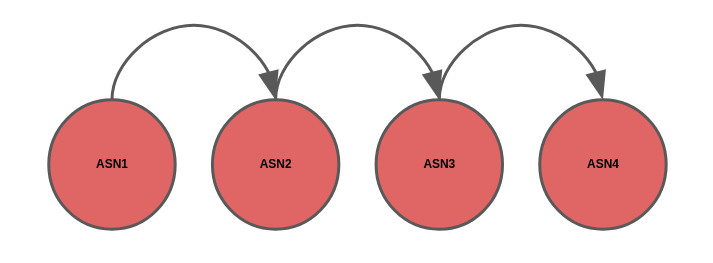
\includegraphics[width=0.5\textwidth]{img/metodologia/aspath_eejmplo_saltos.png}
    \caption{Ejemplo de camino seguido por un paquete según un AS\_PATH}
    \label{fig:aspath_eejmplo_saltos}
\end{figure}

\textbf{¿Por qué no se asume automáticamente que todas las conexiones son bidireccionales?}\\


Porque la existencia de una ruta en una dirección (por ejemplo, de ASN1 a ASN4) no garantiza que el camino inverso exista o sea utilizado. Aunque en la práctica la comunicación IP requiere que haya retorno, BGP no asegura que ese camino de vuelta sea idéntico. Para que se asuma bidireccionalidad, se debe observar también el AS\_PATH inverso explícitamente en el archivo, es decir:\\

\begin{lstlisting}[language=Python, caption=Ejemplo del camino inverso, label=code:formato_sanitized_rib_alreves]
ASN4|ASN3|ASN2|ASN1
\end{lstlisting}


La Figura~\ref{fig:aspath_ejemplos} muestra dos escenarios: (a) cuando se observa la ruta inversa, lo que indica que existe el mismo camino en sentido contrario, y (b) cómo se vería el grafo cuando se observan ambas rutas, permitiendo inferir conexión bidireccional entre los ASes.\\


\begin{figure}[h]
    \centering
    \begin{subfigure}[b]{0.45\textwidth}
        \centering
        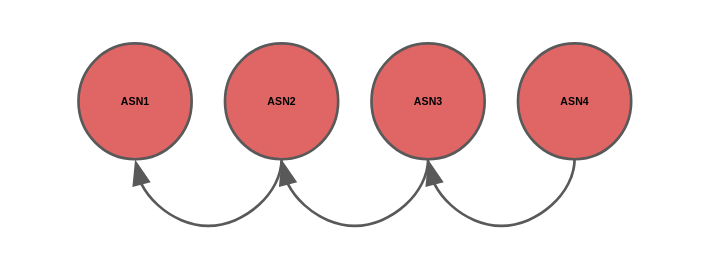
\includegraphics[width=\textwidth]{img/metodologia/aspath_eejmplo_saltos_alreves.png}
        \caption{Ruta observada en dirección inversa}
        \label{fig:aspath_eejmplo_saltos_alreves}
    \end{subfigure}
    \hfill
    \begin{subfigure}[b]{0.45\textwidth}
        \centering
        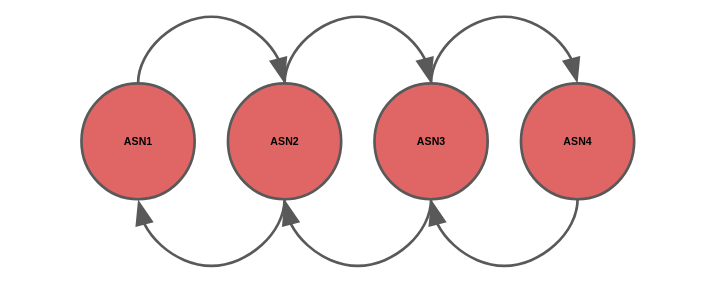
\includegraphics[width=\textwidth]{img/metodologia/aspath_eejmplo_saltos_doble.png}
        \caption{Topología resultante cuando existen ambas rutas}
        \label{fig:aspath_eejmplo_saltos_doble}
    \end{subfigure}
    \caption{Ejemplos de caminos posibles entre ASes según los AS\_PATHs observados}
    \label{fig:aspath_ejemplos}
\end{figure}

Algo importante de destacar y no confundir es que las conexiones entre ASes dadas por el AS\_PATH no están relacionadas directamente con el intercambio de mensajes BGP. La comunicación BGP entre ASes vecinos siempre es bidireccional, pero eso no implica que los AS\_PATHs observados lo sean. De otra forma, los AS\_PATHs representan rutas hacia prefijos, no las sesiones de comunicación BGP entre vecinos.

Una vez comprendida la lógica de la direccionalidad de las conexiones entre ASes dados por las RIBs, se continuó  con la construcción del grafo de Internet a partir de los datos de enrutamiento disponibles.\\

Como se mencionó previamente, en un comienzo se contaba únicamente con atributos de los ASes para la fecha 01/07/2022, extraídos del trabajo~\cite{BenchmarkingGNN}. Sin embargo, esta restricción limitaba los experimentos a una única fecha. Por esta razón, se decidió construir un conjunto de datos propios que permitiese generar atributos de los ASes para distintas fechas, según las necesidades. Sin embargo, esta tarea fue abordada más adelante en el trabajo, una vez obtenidos resultados preliminares sobre el funcionamiento de las GNNs en la tarea planteada. Esto se debió a que no era el foco principal en las primeras etapas.

Lo primero que se buscó fue encontrar una forma eficiente de almacenar la topología del grafo. Si bien, una vez obtenidas las RIBs en los archivos correspondientes, era posible construir el grafo utilizando bibliotecas como NetworkX o DGL, el proceso de leer los archivos y crear el grafo tomaba un tiempo considerable en cada ejecución. Esto se debía recorrer el archivo de las RIBs línea a línea, extrayendo cada ruta para construir de forma incremental la estructura del grafo. Adicionalmente a esto, se le debía sumar una segunda etapa, en la que se incorporaban los atributos de los nodos desde un archivo \texttt{.csv}, lo que añadía un tiempo de procesamiento adicional. Por esta razón, se buscó alguna alternativa para guardar de forma eficiente el grafo junto con sus atributos. Así se optó por utilizar el formato de almacenamiento de \textit{datasets} que ofrece DGL, el cual permite guardar la estructura del grafo con sus respectivos atributos y reutilizarlo en futuras ejecuciones de manera rápida.\\

La biblioteca DGL es una biblioteca diseñada para el fácil uso y manipulación de modelos de Redes Neuronales de Grafos (GNNs). Para guardar un grafo como dataset en el formato que propone la documentación de DGL, se crearon cuatro archivos que definen su estructura y los atributos de los nodos y aristas, según sea necesario. Estos archivos son:

\begin{itemize}
    \item Un archivo \textbf{meta.yaml} que indica qué archivo corresponde a los nodos, aristas y grafos.
    \item Un archivo \textbf{graphs.csv} que asocia un id con diferentes grafos.
    \item Un archivo \textbf{nodes.csv} con los nodos, sus atributos y el id del grafo al que pertenecen.
    \item Un archivo \textbf{edges.csv} con las aristas, sus propiedades y el id del grafo al que pertenecen.
\end{itemize}

















Un extracto del contenido de los archivos \textbf{edges.csv} (Código~\ref{code:contenido_edges}) y \textbf{nodes.csv} (Código~\ref{code:contenido_nodes}) se puede ver a continuación. En el primer caso, se incluyen cuatro columnas: la primera indica a qué grafo pertenece la adyacencia, las dos siguientes corresponden a los ASN (Autonomous System Number, por sus siglas en inglés) que representan la existencia de una relación direccional entre dos ASes, y la cuarta columna señala el tipo de relación que comparten, según el formato definido en~\ref{code:formato_out_benchmark}. En cuanto al segundo archivo, contiene tres columnas: la primera identifica el grafo al que pertenece el nodo, la segunda a un identificador del nodo (en este caso, el ASN del Sistema Autónomo) y la tercera columna almacena un string con todos los atributos asociados a dicho nodo, separados por una coma.\\


\begin{lstlisting}[language=Python, caption=Extracto contenido archivo edges.csv, label=code:contenido_edges]
graph_id,src_id,dst_id, Relationship
0,28792,6939,0
0,28792,3257,1
0,28792,9318,0
\end{lstlisting}

\begin{lstlisting}[language=Python, caption=Extracto contenido archivo nodes.csv, label=code:contenido_nodes]
graph_id,node_id,feat
0,28792,"0.2842043341251542, 0.2928342377832154, 0.3340535381175178, 0.2554473035666517, 0.0, 0.0, 1.0, 0.0, ... ,
...
\end{lstlisting}


% Explciar el codigo de crear grafo la clase q crea primero el grafo despeus agrega los attr pero esa se demora pero guaad en libreia dgl pero despues dse llama y es super rapdio ocuapr el grafo

Como se explicó previamente, leer los archivos RIBs toma tiempo, y hacerlo repetidamente no es eficiente. Por esta razón, se optó por utilizar el formato de almacenamiento descrito anteriormente (formato de \textit{datasets} de la biblioteca DGL). Sin embargo, una vez generado el archivo \texttt{sanitized\_rib.txt}, es necesario recorrerlo al menos una vez línea por línea para poder construir los tres archivos descritos (\texttt{nodes.csv}, \texttt{edges.csv} y \texttt{meta.yaml}). Para facilitar este proceso se creó una clase específica encargada de crear el grafo~\ref{code:cclase_graph}.\\

\begin{lstlisting}[language=Python, caption=Extracto clase Graph encargada de la construcción de la creación de archivos formato DGL. , label=code:cclase_graph]
class Graph:
    def __init__(self,dataset_graph_path ,max_paths,debug = False):
        self.debug = debug
        self.nx_graph = None
        self.data_path = dataset_graph_path
        
    def create_topology_from_ribs(self, rib_filename:str,filename_out="edges.csv"):
        ...
    def features_nodes(self,features_filename,filename_out="nodes.csv"):
        ...
    def remove_nodes_degree(self, degree,filename_out="edges.csv"):
        ...
...
\end{lstlisting}

\newpage
Esta clase se encarga primero de crear la topología del grafo, es decir, leer el archivo con las RIBs y generar los archivos \textbf{edges.csv} y \textbf{nodes.csv}. Una vez construida la estructura base, la clase cuenta con distintos métodos que permiten agregar atributos a los nodos según los experimentos realizados (Sección~\ref{sec:gnn_result_section}). Algunos ejemplos de atributos utilizados son métricas de centralidad como el grado del nodo, el uso del dataset mencionado previamente que ya contenía atributos para ASes en una fecha específica (detallados en la Tabla~\ref{tab:as_attr_tabla_bechmark}) , y también un conjunto de atributos generado por nosotros para otras fechas, adaptado a las necesidades del estudio (detallado en Tabla~\ref{tab:as_attr_tabla} ) .\\
 
Por último, se incluyó en el código la opción de eliminar nodos cuyo grado sea igual a un valor especificado, con el objetivo de remover nodos hoja (es decir, aquellos con grado igual a 1) que se ubican en la periferia del grafo de Internet. Esta operación puede repetirse durante una cantidad determinada de iteraciones, lo que permite simplificar la topología del grafo según los requerimientos de los distintos experimentos realizados.\\

Una vez ejecutado el bloque de código, se obtiene la siguiente estructura de carpetas y archivos, como se muestra en la Figura~\ref{repo_grap_dataset}:\\

\begin{lstlisting}[basicstyle=\ttfamily,label=repo_grap_dataset ,frame=single, caption=Estructura del repositorio del \textit{benchmark}]
dgl_graph/
    graphs.csv
    nodes.csv
    edges.csv
    meta.yaml
\end{lstlisting}

Como se mencionó en la Sección~\ref{sec:obtencion_datos_section}, en un comienzo se trabajó únicamente con los atributos de ASes extraídos del dataset utilizado en el trabajo de Giakatos et al.~\cite{BenchmarkingGNN}. Para poder utilizar esta información de manera adecuada, se desarrolló un código automatizado que permitiera identificar la fecha a la que correspondían dichos atributos. Esto se logró comparando la topología de Internet utilizada en el estudio con las topologías disponibles en el repositorio de CAIDA\cite{CAIDAS-relationship} (mismo repositorio con el que este estudio trabajó), correspondientes a diferentes fechas.\\

Para ello, se descargaron los archivos de CAIDA que contienen las conexiones entre ASes para cada mes desde 2020, considerando tanto los conjuntos serial-1 como serial-2. A partir de estos archivos, se construyó un grafo para cada fecha y se comparó su estructura con la topología utilizada en el estudio. Finalmente, se identificó la coincidencia con la topología correspondiente a julio de 2022, concluyendo que el dataset de atributos de ASes empleado en el trabajo hace referencia a esa fecha.\\

Más adelante en el trabajo, cuando se contó con un mayor conocimiento sobre los Sistemas Autónomos, así como sobre los distintos \textit{datasets} y fuentes de información pública disponibles en Internet sobre el tema, se decidió construir un conjunto propio de atributos de ASes. Esto con el objetivo de analizar y evaluar si tenían un impacto significativo en los resultados obtenidos durante los experimentos, además de evitar la limitación de fecha que se tenía para los experimentos.\\

\begin{lstlisting}[language=Python, caption=Ejemplo de mapeo de ASN a índices para entrenamiento y prueba en BGP2Vec., label=code:formato_sanitized_rib]
# ASN a índice -> x_training y x_test
x_training_mapped = []
y_training_filtered = []

# Recorrer pares (asn, asn) y agregar sólo los válidos
for (a, b), y in zip(x_training, y_training):
    a_index = asn_to_index.get(str(a), 0)
    b_index = asn_to_index.get(str(b), 0)

    # Ignorar si índice es 0 
    if a_index == 0 or b_index == 0:
        continue
    
    x_training_mapped.append([a_index, b_index])
    y_training_filtered.append(y)

# Convertir listas a arrays de NumPy
x_training_mapped = np.array(x_training_mapped)
y_training_filtered = np.array(y_training_filtered)

# ---------------------------------------------------------------------------

x_test_mapped = []
y_test_filtered = []

for (a, b), y in zip(x_test, y_test):
    a_index = asn_to_index.get(str(a), 0)
    b_index = asn_to_index.get(str(b), 0)

    # Ignorar si índice es 0 
    if a_index == 0 or b_index == 0:
        continue
    
    x_test_mapped.append([a_index, b_index])
    y_test_filtered.append(y)

x_test_mapped = np.array(x_test_mapped)
y_test_filtered = np.array(y_test_filtered)
\end{lstlisting}


\subsection{Atributos extraídos de PeeringDB} \label{sec:Atributos_extraidos_PeeringDB}

Para la obtención de atributos para los Sistemas Autónomos se utilizaron los datos de PeeringDB~\cite{PeeringDB}, un esfuerzo colaborativo donde administradores de Sistemas Autónomos aportan información sobre sus redes. Más información sobre PeeringDB puede encontrarse en el Anexo~\ref{sec:anexo_recoleccion_datos_internet}.\\

%este análisis se encuentra en el Anexo~\ref{sec:estudio_attr_peeringdb_anexo}

Para decidir los atributos más relevantes para este trabajo, primero se realizó un análisis exploratorio de los datos disponibles en PeringDB, con el objetivo de comprender el tipo de información ofrecida y su posible utilidad para la tarea de inferencia (este estudio se encuentra detallado en el Anexo~\ref{sec:anexo_exploracion_datos_peeringdb}). Luego, se llevó a cabo la preparación de los datos, que incluyó la limpieza del conjunto de datos y el tratamiento de atributos faltantes. En esta etapa, se identificaron dos tipos principales de atributos: numéricos y categóricos.\\



En el caso de los atributos categóricos, estos fueron transformados a vectores one-hot. Por otro lado, para los atributos numéricos, con el fin de homogeneizar sus rangos y reducir la variabilidad, se aplicó la función $x \rightarrow \log{(x+1)}$ y para normalizar se utilizó $x \rightarrow \frac{x - \min(x)}{\max(x) - \min(x)}$. \\

%Finalmente, para identificar las variables más relevantes para el modelo, se aplicó un proceso de selección de características....\\

% Hablar sobre pageRank

En la Tabla~\ref{tab:as_attr_tabla} se muestran los atributos que se incorporaron a los Sistemas Autónomos:\\

% TODO: Cambiar valores de los atributos numericos a como estaban antes.

\begin{table}[ht]

\centering

\footnotesize

\rowcolors{2}{grayA}{grayB}  % ← intercalado entre grisA y grisB

\begin{tabular}{|p{3.6cm}|p{6.8cm}|p{4cm}|}

\hline

\rowcolor{white}  % encabezado blanco

\textbf{Atributos} & \textbf{Descripción} & \textbf{Tipo de dato} \\

\hline

ix\_count & Cantidad de IXPs donde el AS está presente & Numérico $\in [0,1] $\\

fac\_count & Número de instalaciones donde opera & Numérico $\in [0,1]$ \\

info\_prefixes4 & Cantidad de prefijos IPv4 que anuncia la red & Numérico $\in [0,1]$ \\

info\_prefixes6 & Cantidad de prefijos IPv6 que anuncia la red & Numérico $\in [0,1]$ \\

policy\_general & Política de peering & Numérico $\in [0,1]$ \\

policy\_locations & Lugares donde aplica la política de peering & Categórico (6 categorías) \\

policy\_contracts & Requiere contrato para establecer una relación de peering& Categórico (4 categorías) \\

info\_traffic & Nivel estimado de tráfico & Categórico (19 categorías) \\

info\_scope & Alcance de la red & Categórico (11 categorías) \\

info\_type & Tipo de red & Categórico (12 categorías) \\

info\_ratio & Proporción de tráfico entrante y saliente de la red & Categórico (7 categorías) \\

PageRank & Importancia estructural del AS según su conectividad en la red & Numérico $\in[0, 6.76 \times 10^{-5}]$ \\ %ver si arreglar

\hline

\end{tabular}

\caption{Atributos considerados para representar los nodos (ASes) en la construcción del grafo.}

\label{tab:as_attr_tabla}

\end{table}


% TODO: Ver si incorporar -> Cabe destacar que para muchos ASes no se encontrba informacion, por lo que estos eran completados ? 

Con esta información se generó un archivo \texttt{.csv} que contiene los atributos de cada AS para un mes determinado, con los valores ya normalizados. Este archivo fue utilizado posteriormente al momento de construir el grafo y el dataset de la topología de Internet correspondiente a los primeros meses del año 2024.\\

%-----------------------------------------------------------------------------------------------------------------------------------------------------------------------------------------------------
\section{GNN} \label{sec:gnn_section}

Luego de creado el dataset correspondiente al grafo de Internet, se comenzó a abordar la tarea de inferencia utilizando Redes Neuronales de Grafos (GNN), donde se adoptaron dos enfoques:

\begin{enumerate}

    \item \textbf{Entrenamiento por etapas}: En este enfoque, el pipeline se divide en dos etapas. La primera, donde se aprenden las representaciones de los nodos (embeddings) utilizando GNNs. Y la segunda, donde estas representaciones se utilizan como entrada para una Red Neuronal Artificial (ANN), que actúa como clasificador para realizar la tarea de inferencia.
    
    \item \textbf{Entrenamiento end-to-end}: En este segundo enfoque, el modelo GNN aprende las representaciones de los nodos —es decir, se entrena— con base en la tarea específica, en este caso, la clasificación de aristas.  
    
    % puede causar overfitting?
    

\end{enumerate}

En ambos enfoques se tomó un esquema encoder-decoder, donde la GNN actúa como codificador (\textit{encoder}), generando representaciones vectoriales para cada nodo, las que son luego utilizadas por un decodificador (\textit{decoder}), cuya implementación varía según la tarea y el enfoque utilizado. \\

Las arquitecturas de GNNs que se utilizaron fueron: GCN (Graph Convolutional Network), GraphSAGE (SAmple and aggreGatE) y GAT (Graph Attention Network). Como \textit{decoder}, se utilizó una MLP (Multilayer Perceptron) en ambos enfoques. También, en el enfoque por etapas se ocupó un decodificador basado en producto punto (Dot Product) para la tarea de predicción de enlaces, mientras que en el enfoque end-to-end se consideró también un decodificador Bilinear para la clasificación de relaciones.\\ 
%(Más información sobre los decoders utilizados en ANEXO\ref{anexo:decoders}).\\




En el Codigo~\ref{code:modelo_gcn} correspondiente a una clase que implementa un modelo basado en GCN. En este ejemplo, el método \textit{encode} realiza el forward pass, correspondiente a las dos capas GNN, mientras que los métodos \textit{decodeDotProduct}, \textit{decodeMLP} y \textit{decodeBilinear} actúan como \textit{decoders}.\\

\begin{lstlisting}[language=Python, caption=Ejemplo modelo GraphSAGE , label=code:modelo_gcn]
class GCN(nn.Module):
    def __init__(self, in_feats, hidden_feats, out_feats, out_feats_mlp=1, drop=0.3):
        super().__init__()
        self.conv1 = GraphConv(in_feats, hidden_feats)
        self.conv2 = GraphConv(hidden_feats, out_feats)
    
        self.MLP = MLPPredictor(out_feats,out_feats_mlp)
        self.BilinearDecoder = BilinearPredictor(out_feats, 3)
        self.regressor = nn.Linear(out_feats, 1)
        self.drop  = nn.Dropout(drop)           


    def encode(self, g, x):
        g = dgl.add_self_loop(g)
        h = self.drop(F.relu(self.conv1(g, x)))  
        h = self.conv2(g, h)                     
        return h

    
    def decodeDotProduct(self, g, h):
        with g.local_scope():
            g.ndata["h"] = h
            # Compute a new edge feature named 'score' by a dot-product between the
            # source node feature 'h' and destination node feature 'h'.
            g.apply_edges(fn.u_dot_v("h", "h", "score"))
            # u_dot_v returns a 1-element vector for each edge so you need to squeeze it.
            return g.edata["score"][:, 0]
        
    def decodeMLP(self, g, h):
        return self.MLP(g, h)  
    
    def decodeBilinear(self, g, h):
        return self.BilinearDecoder(g, h)

    def forward(self, g, x):
        h = self.encode(g, x)  # Embeddings
        out = self.regressor(h).squeeze(-1)  # Predicción final
        return out 
        
\end{lstlisting}

Cabe mencionar que en el entrenamiento en Redes Neuronales de Grafos existen diferentes modalidades para entrenar un modelo, dependiendo de cómo se utilicen los nodos y el grafo durante el entrenamiento e inferencia.\\


%existen diferentes modalidades para entrenar un modelo, en primera instancia en cómo se utilizan los nodos y el grafo durante el entrenamiento e inferencia:\\

\begin{itemize}
    \item \textbf{Inductivo:} El conjunto de entrenamiento y el de prueba están completamente separados, es decir, se trabaja con grafos distintos. Este enfoque permite una mejor generalización, ya que el modelo debe generar predicciones sobre nodos y estructuras que no ha visto antes. Sin embargo, una desventaja es que no siempre se cuenta con múltiples grafos para poder entrenar y evaluar el modelo.
    
    \item \textbf{Transductivo:} Se tiene un único grafo que se usa tanto para el entrenamiento como para la inferencia. Sin embargo, la función de pérdida se calcula solamente sobre los nodos que se definieron como parte del conjunto de entrenamiento. Este enfoque es útil cuando se cuenta con un único grafo completo y se debe predecir información específica dentro del mismo.\\
    
\end{itemize}

Para trabajar con estos enfoques y nuestros datos, la separación del grafo en entrenamiento y test se trabajó de la siguiente forma:

\begin{itemize}

    \item \textbf{Usar el grafo completo con pérdida filtrada (enfoque transductivo):} \\
    En este caso se utiliza el grafo completo durante el entrenamiento, pero la función de pérdida se calcula solo sobre los elementos del conjunto de entrenamiento (ya sean nodos o aristas).
    Se aplicó en dos casos:
    \begin{itemize}
        \item \textbf{Clasificación de aristas} (en el enfoque end-to-end)
        \item \textbf{Predicción de atributos de nodos} (en el enfoque por etapas para la generación de embeddings)
    \end{itemize}
    
    \item \textbf{Crear subgrafos separados (enfoque inductivo):} \\
    Se generan dos subgrafos separados a partir del grafo principal, uno para el entrenamiento y otro para la validación, eliminando las aristas correspondientes.\\
    Se aplicó en el caso:
    \begin{itemize}
        \item \textbf{Predicción de aristas} (en el enfoque por etapas). Evita que el modelo tenga acceso a las aristas que luego debe predecir, reduciendo el riesgo de fuga de información.
    \end{itemize}
\end{itemize}


% \usepackage{booktabs}
% \usepackage{tabularx}


% Paquetes recomendados en el preámbulo:
% \usepackage{array,longtable,booktabs,enumitem}
% Definir un tipo de columna alineada a la izquierda con ancho fijo:
\newcolumntype{P}[1]{>{\raggedright\arraybackslash}p{#1}}

\begin{longtable}{P{0.27\textwidth} P{0.45\textwidth} P{0.24\textwidth}}
\caption{Estrategias de entrenamiento de los datos según la tarea con GNN.}
\label{tab:division_grafo_estrategias_long} \\
\toprule
\textbf{Estrategia} & \textbf{Descripción} & \textbf{Se aplicó en} \\
\midrule
\endfirsthead
\toprule
\textbf{Estrategia} & \textbf{Descripción} & \textbf{Se aplicó en} \\
\midrule
\endhead

Grafo completo con pérdida filtrada
&
Se usa el grafo completo durante el entrenamiento, pero la función de pérdida se calcula \emph{solo} sobre los elementos del conjunto de entrenamiento (nodos o aristas).
&
\begin{itemize}[leftmargin=*,nosep]
  \item Clasificación de aristas (enfoque end-to-end).
  \item Predicción de atributos de nodos (enfoque por etapas para generar \textit{embeddings}).
\end{itemize}
\\
\addlinespace
Subgrafos separados (train/valid)
&
Se generan dos subgrafos disjuntos (entrenamiento y validación) eliminando las aristas correspondientes. Evita que el modelo acceda a aristas que luego debe predecir, reduciendo la fuga de información.
&
Predicción de aristas (enfoque por etapas).
\\
\bottomrule
\end{longtable}


%Otro aspecto adicional fue que para evitar fuga de información, incluir ambas aristas dirigidas de un mismo par de nodos dentro de el mismo conjunto de entrenamiento o validación.\\


Una vez definidos los conjuntos de entrenamiento y validación, se procedió al entrenamiento de los modelos. Para ello, se trabajó con \textit{early stopping} para evitar sobreajuste. Además, se monitorearon métricas como la pérdida y la Accuracy a lo largo de los epochs, y se evaluó el rendimiento final mediante el uso de matrices de confusión y las métricas de evaluación. 































%/////////////////////////////////////////////////////////////////////
% SEGUNDO ENFOQUE: EMB+TASK--------------------------------------

\subsection{Primer Enfoque: \textit{Por etapas} }



Como se mencionó anteriormente, se trabajó con dos enfoques de flujo de entrenamiento. 
El primero, denominado \textit{por etapas}, es más útil cuando se dispone de un conjunto de datos de etiquetado limitado o para generar representaciones que luego serán utilizadas para diferentes tareas (\textit{downstream task}). 
En este esquema hay dos etapas: primero, se aprenden las representaciones de los nodos. Luego, estas representaciones son utilizadas como entrada a una ANN que actúa como clasificador. Para este caso se suele tener un rendimiento inferior en comparación con el enfoque \textit{end-to.end}, sin embargo, al ser las representaciones más genéricas, pueden utilizarse para múltiples tareas.\\


En la Figura~\ref{fig:diagrama-de-flujo-efoque2} se muestra el flujo general de este enfoque. La entrada consiste en las rutas BGP previamente sanitizadas (\texttt{sanitized\_ribs.txt}), a partir de las cuales se construye la topología del grafo de Internet. Luego, una GNN genera embeddings a partir de la información estructural y de atributos de los nodos —la selección de estos atributos se detalla más adelante—. Estas representaciones son luego utilizadas como entrada para una ANN, encargada de inferir la relación entre pares de nodos.\\

\begin{figure}[h]
    \centering
    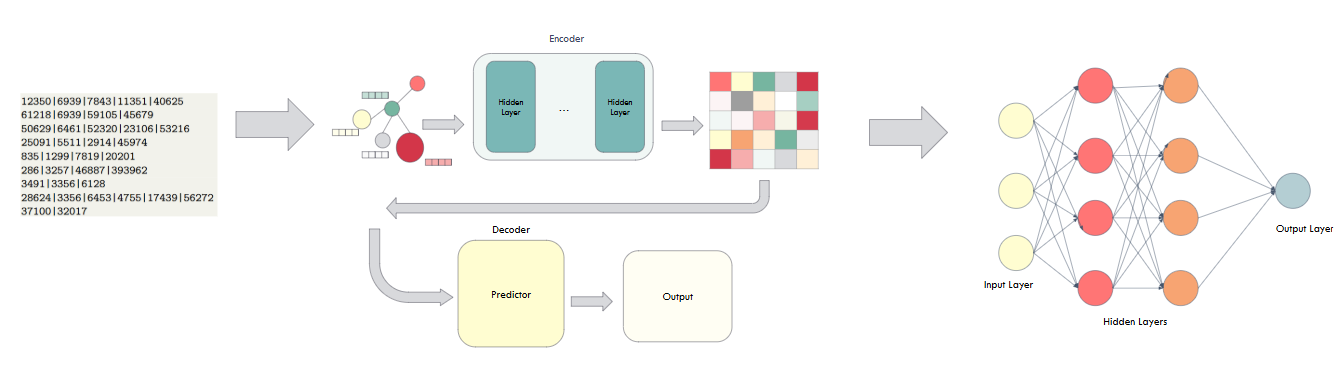
\includegraphics[width=1\textwidth]{img/gnn/gnn-enfoque-2.png}
    \caption{Diagrama de flujo del primer enfoque: Entrenamiento de embeddings de nodos para luego pasar la entrada a una ANN para la tarea de clasificación}
    \label{fig:diagrama-de-flujo-efoque2}
\end{figure}

%TODO: Agregar en inform eq esto se agregó
\begin{algorithm}[H]
\caption{Entrenamiento por etapas para inferencia de relaciones entre ASes}
\label{alg:gnn_por_etapas}
\begin{algorithmic}[1]
\Require Grafo $G$, atributos de nodos $X$, tarea auxiliar $T$, pares etiquetados $(u,v,y)$
\Ensure Clasificador entrenado para inferencia de relaciones
\State Inicializar encoder GNN
\State Entrenar la GNN sobre la tarea auxiliar $T$
\State Obtener embeddings de nodos $H$
\State Construir vectores de entrada para pares $(u,v)$ a partir de $H$
\State Entrenar un clasificador supervisado sobre las etiquetas $y$
\State Evaluar el clasificador sobre el conjunto de prueba
\end{algorithmic}
\end{algorithm}

El flujo general del enfoque por etapas se resume en el Algoritmo~\ref{alg:gnn_por_etapas}.





Las tareas utilizadas para crear las representaciones vectoriales de los Sistemas Autónomos en el grafo de Internet fueron:\\

\begin{enumerate}

    \item \textbf{Predicción de existencia de arista entre nodos}: Se trabajó sobre una tarea binaria, donde se entrenó al modelo para distinguir si dos pares de nodos estaban conectados o no (generando aristas negativas). Esto permite que los embeddings capturen patrones de conectividad entre los nodos.

    \item \textbf{Predicción de atributos}: El modelo se entrena para predecir propiedades específicas de los nodos, en este caso, su \textit{grado} y su valor de \textit{PageRank}. El objetivo de esto es hacer que la GNN aprenda representaciones que reflejen la posición y el rol estructural de cada nodo dentro del grafo.

\end{enumerate}




Para la segunda etapa correspondiente a la predicción de relaciones, se utilizó una Red Neuronal que recibe como entrada los embeddings de dos nodos adyacentes. Esta red combina la información de ambos nodos y retorna una predicción sobre el tipo de relación existente entre ellos. Sin embargo, antes de trabajar directamente con los datos de entrenamiento y evaluación, fue necesario adaptarlos para que pudieran ser utilizados junto a los embeddings generados previamente por la GNN. Para esto, se creó un diccionario que asignaba un ID a cada ASN, de forma que los embeddings pudieran ser asociados de manera consistente. Los IDs fueron definidos en base al valor de los ASN, para de esta forma facilitar la interpretación de los resultados y mantener una trazabilidad más simple.\\



Dado que los modelos de embeddings trabajan con IDs en lugar de valores simbólicos como los ASN (forma en que nuestro dataset ToR era identificado), se tuvo que adaptar el conjunto de entrenamiento y prueba. Específicamente, se mapeó cada ASN a un ID utilizando un diccionario que se creó previamente en el trabajo, si alguno de los ASN no era encontrado en dicho diccionario (es decir, no tenía un ID asociado), el nodo era descartado del conjunto (Código~\ref{code:mapeo_asn_id}).\\



%, si alguno de los ASN no se encontraba en los conjuntos, no se encontraba presente en el diccionario (es decir, no tenía un ID asociado); este ejemplo se descartaba del conjunto (Código~\ref{code:mapeo_asn_id}). \\



\begin{lstlisting}[language=Python, basicstyle=\ttfamily\footnotesize, label=code:mapeo_asn_id, frame=single, caption={Modelo CNN utilizado en el enfoque BGP2VEC para clasificación de relaciones AS.}]
# Mapeo de ASN a índices para conjuntos de entrenamiento
x_training_mapped = []
y_training_filtered = []

# Recorrer cada par (asn, asn) en entrenamiento y filtrar válidos
for (a, b), y in zip(x_training, y_training):
    a_index = asn_to_index.get(str(a), 0)
    b_index = asn_to_index.get(str(b), 0)

    # Ignorar si alguno de los índices es 0 (no mapeado)
    if a_index == 0 or b_index == 0:
        continue

    x_training_mapped.append([a_index, b_index])
    y_training_filtered.append(y)

# Convertir a arreglos NumPy
x_training_mapped = np.array(x_training_mapped)
y_training_filtered = np.array(y_training_filtered)

# ---------------------------------------------------------------------------
# Mismo proceso para el conjunto de prueba
x_test_mapped = []
y_test_filtered = []

for (a, b), y in zip(x_test, y_test):
    a_index = asn_to_index.get(str(a), 0)
    b_index = asn_to_index.get(str(b), 0)

    if a_index == 0 or b_index == 0:
        continue

    x_test_mapped.append([a_index, b_index])
    y_test_filtered.append(y)

x_test_mapped = np.array(x_test_mapped)
y_test_filtered = np.array(y_test_filtered)

# Guardar los datos procesados
np.save(PATH + DATA + "x_training_mapped.npy", x_training_mapped)
np.save(PATH + DATA + "y_training_filtered.npy", y_training_filtered)
np.save(PATH + DATA + "x_test_mapped.npy", x_test_mapped)
np.save(PATH + DATA + "y_test_filtered.npy", y_test_filtered)
\end{lstlisting}




La Red Neuronal utilizada en esta etapa fue la misma propuesta en el enfoque BGP2Vec para la clasificación de relaciones entre Sistemas Autónomos. Este modelo se basa en una arquitectura de \textit{Convolutional Neural Network (CNN)}. La entrada corresponde a secuencias de pares de identificadores, correspondientes a los ASN involucrados. Estos IDs son transformados en sus representaciones vectoriales mediante una capa de tipo \textit{Embedding}, la cual puede estar fija (no entrenable) o entrenarse junto al modelo, dependiendo del experimento. Luego, se aplican capas convolucionales para extraer patrones espaciales en las representaciones, seguidas por capas de \textit{MaxPooling}, \textit{Flatten} y, finalmente, capas densas que concluyen en una función \textit{softmax} para obtener una salida única que corresponde a la clase predicha.\\

\newpage
A continuación se muestra el código correspondiente a la implementación del modelo:\\





\begin{lstlisting}[basicstyle=\ttfamily, label=code:cnn_bgp2vec_model, frame=single, caption=Modelo CNN utilizado en el enfoque BGP2VEC para clasificación de relaciones AS.]
# Configuración de la red BGP2VEC
experiment = None
num_classes = len(class_names)
embedding_trainable = False
input_length = 2  # Longitud de la secuencia de entrada
embedding_vector_length = embeddings.shape[1]  # Dimensión de los vectores de embedding
total_ASNs = embeddings.shape[0]  # Tamaño del vocabulario (número de ASes)

# Definición del modelo
model = Sequential()
model.add(Embedding(total_ASNs, embedding_vector_length, input_length=input_length,
                    weights=[embeddings], trainable=embedding_trainable))
model.add(Conv1D(filters=32, kernel_size=3, padding='same', activation='relu'))

model.add(Reshape((32, 2)))  # Ajuste necesario de dimensiones para la siguiente capa
model.add(MaxPooling1D(pool_size=2))

model.add(Conv1D(filters=32, kernel_size=3, padding='same', activation='relu'))
model.add(Reshape((32, 16)))  # Nuevo ajuste de dimensiones
model.add(MaxPooling1D(pool_size=2))

model.add(Flatten())
model.add(Dense(100, activation='relu'))
model.add(Dense(num_classes, activation='softmax'))
\end{lstlisting}

Una breve explicación de las demás capas utilizadas en esta arquitectura, además de las convoluciones:\\

\begin{itemize}

    \item \textbf{MaxPooling1D:} Reduce la dimensión de la salida de una capa convolucional tomando el máximo valor dentro de una ventana deslizante sobre la secuencia de datos.

    \item \textbf{Flatten:} Toma una entrada multidimensional (por ejemplo, una matriz o un tensor 3D) y la aplana en un vector 1D. Convierte la salida de las capas convolucionales y de pooling en un formato que pueda ser usado por las capas densas (Dense).

    \item \textbf{Dense:} Es una capa completamente conectada (fully connected), donde cada neurona está conectada a todas las salidas de la capa anterior.

    \item \textbf{Función softmax:} Convierte el vector de valores reales (logits) en un vector de probabilidades, donde cada valor queda entre 0 y 1 y la suma de ellos es 1.\\

\end{itemize}

Un problema que se conocía desde el inicio, y que se hizo especialmente evidente a partir de los primeros resultados del modelo, fue el del desbalance de clases presente en el dataset. Este se evidencia en la Figura~\ref{fig:relaciones_por_tipo_asrank} donde se observa que hay una cantidad considerablemente mayor de relaciones P2P que de C2P.\\

%Esto también se aprecia en los resultados obtenidos, como se muestra en las Figuras ~\ref{fig:anex:matrices_confusion_experimentos_gnns_decoder}  correspondientes a las matrices de confusión para diferentes experimentos.\\

Para trabajar este problema, se calcularon pesos específicos para cada clase en función de su frecuencia en el conjunto de entrenamiento. Con estos valores se crea un diccionario \texttt{class\_weight\_dict}, el cual se utiliza para ajustar la función de pérdida para las diferentes clases, asignando mayor peso a las clases menos representadas y menor peso a las clases más frecuentes (Código~\ref{code:class_weights_dict}).\\

\begin{lstlisting}[basicstyle=\ttfamily, label=code:class_weights_dict, frame=single, caption=Estructura del repositorio de los experimentos para la tarea de inferencia usando GNNs]
from sklearn.utils import class_weight
import numpy as np

class_weights = class_weight.compute_class_weight(
                    class_weight='balanced', 
                    classes=np.array(list(range(num_classes))), 
                    y=y_training_filtered)

class_weight_dict = {i: w for i, w in enumerate(class_weights)}
# {0: 0.49730749665083795, 1: 2.020894588161655, 2: 2.0228938408395782}
print('[class_weights_dict]:', class_weight_dict)
\end{lstlisting}

También se decidió generar representaciones vectoriales (embeddings) de los nodos utilizando el algoritmo \textbf{DeepWalk}, para comparar su desempeño respecto a los embeddings generados por la GNN. A diferencia de las GNN, DeepWalk se basa únicamente en la estructura del grafo.\\




%/////////////////////////////////////////////////////////////////////
%/////////////////////////////////////////////////////////////////////
% Segundo ENFOQUE: END-TO-END --------------------------------
\subsection{Segundo Enfoque: \textit{end-to-end} }
\label{sec:SegundoEnfoque}
Este enfoque (\textit{end-to-end}) es útil cuando se tiene un conjunto suficiente de datos etiquetados, ya que permite que la GNN aprenda representaciones directamente de la tarea de clasificación. Esto hace que las representaciones aprendidas sean muy específicas, por lo que no siempre pueden reutilizarse en otros contextos.\\

% TODO:Agregar mas citas de donde saco las cosas y a que esepcificamente me refiero

% TODO: Comentar como se hizo el split?
En la Figura~\ref{fig:diagrama-de-flujo-endtoend1}, se observa el flujo de entrenamiento. Como entrada, se entrega el grafo con los respectivos atributos de los nodos y las etiquetas de las relaciones (aristas). El encoder corresponde a arquitecturas GNN, las cuales generan embeddings para cada nodo. Estas representaciones son utilizadas por alguno de los decoders, produciendo así un vector de puntuaciones para cada posible relación. La clase con mayor puntaje es seleccionada como predicción. A partir de este resultado se calcula la función de pérdida, la cual, mediante el backpropagation, ajusta de forma conjunta tanto los parámetros del encoder como del decoder.\\

\begin{figure}[h]

    \centering

    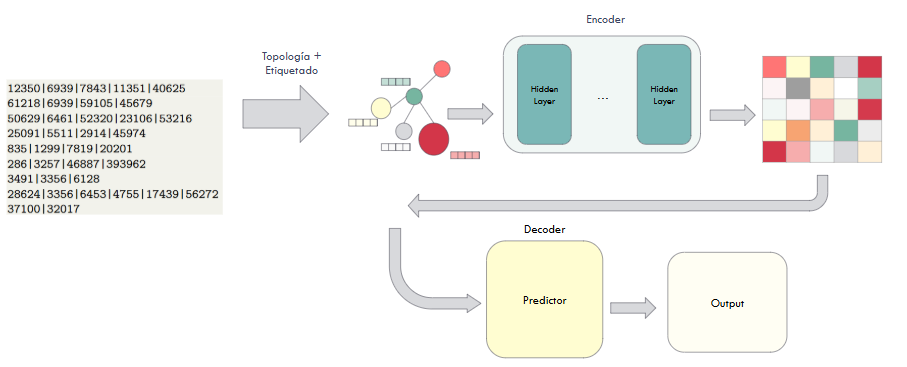
\includegraphics[width=0.9\textwidth]{img/gnn/gnn-endtoend1.png}

    \caption{Diagrama de flujo del entrenamiento \textit{end-to-end}.}

    \label{fig:diagrama-de-flujo-endtoend1}

\end{figure}





%TODO: se agrgo aqui esto infome
\begin{algorithm}[H]
\caption{Entrenamiento end-to-end para clasificación de relaciones entre ASes}
\label{alg:gnn_end_to_end}
\begin{algorithmic}[1]
\Require Grafo $G$, atributos de nodos $X$, aristas etiquetadas $E_L$
\Ensure Modelo encoder-decoder entrenado
\State Inicializar encoder GNN y decoder
\For{cada época}
    \State Generar embeddings de nodos a partir de $G$ y $X$
    \State Predecir etiquetas sobre las aristas de entrenamiento
    \State Calcular la función de pérdida
    \State Actualizar parámetros mediante backpropagation
\EndFor
\State Evaluar el modelo sobre las aristas de validación o prueba
\end{algorithmic}
\end{algorithm}

El flujo general del enfoque end-to-end se resume en el Algoritmo~\ref{alg:gnn_end_to_end}.






Como se mencionó anteriormente, en esta tarea se utilizó el grafo completo para el entrenamiento, pero filtrando las aristas al momento de calcular la función de pérdida, de modo que solo se consideraran aquellas que pertenecían al conjunto de entrenamiento.

En este enfoque, luego de cargar el grafo, se procedió a etiquetar las aristas utilizando el dataset de relaciones provisto por CAIDA. Debido a la baja cantidad de ejemplos disponibles para ciertos tipos de relaciones, se decidió incorporar todas las aristas que se encontraban presentes en el conjunto de datos de CAIDA. Esta decisión permitió ampliar la cantidad de muestras etiquetadas y así facilitar el entrenamiento del modelo en la tarea de clasificación de aristas.\\

Durante esta etapa se realizaron distintas variaciones de experimentos con el objetivo de evaluar el impacto de las decisiones de diseño del modelo. Se probaron diferentes arquitecturas de GNN, combinadas con distintos tipos de decodificadores. Además, se evaluaron distintos esquemas de atributos de nodos: atributos reales sacados de PeeringDB, atributos basados únicamente en el grado de los nodos, y atributos aleatorios.\\

Además, se exploró el uso de técnicas de \textit{sampling}, en particular \texttt{Neighbor Sampling}, donde para cada batch se toma un subconjunto de nodos y un número fijo de vecinos por capa, y \texttt{ClusterGCN}, que agrupa el grafo en pequeños subgrafos (clusters) y entrena sobre ellos por separado.
Se probaron estas técnicas para observar cómo cambia el resultado al entrenar con menos información de la estructura del grafo.\\





.







\subsection{Distribución del Repositorio}

Al igual que en el \textit{benchmark} mencionado previamente (Sección~\ref{sec:Benchmark_section}), en este caso también se utilizó un repositorio distinto en GitHub~\cite{gnnCode} para trabajar y almacenar el código, además de servir como sistema de control de versiones. Permitiendo así trabajar desde diferentes dispositivos.\\


La Figura~\ref{benchmark_repo_estructura} muestra la estructura del repositorio que se utilizó para los experimentos utilizando GNNs. El directorio contiene los datos, los resultados, los módulos implementados y diversos notebooks con los diferentes enfoques que se utilizaron.\\

\begin{lstlisting}[basicstyle=\ttfamily, label=benchmark_repo_estructura, frame=single, caption=Estructura del repositorio de los experimentos para la tarea de inferencia usando GNNs.]
data/
results/
modules/
    gnn_models.py
    gnn.py
    graph.py
AS_relationship_inference_gnn.ipynb
train_embeddings.ipynb
AS_relationship_inference.ipynb
create_as_attr.ipynb
create_graph.ipynb
utils.py
\end{lstlisting}

Dentro del directorio \texttt{data/} se almacenan todos los archivos necesarios para la realización de los experimentos: los embeddings de los Sistemas Autónomos generados durante el entrenamiento, los modelos entrenados, los archivos necesarios para la construcción del grafo de ASes, así como las RIBs ya sanitizadas, los \textit{datasets} con las relaciones entre ASes extraídas de CAIDA y los archivos provenientes de PeeringDB.\\

Por otro lado, el directorio \texttt{results/} almacena los resultados de todos los experimentos realizados. Estos se guardan en archivos \texttt{.csv} con el formato mostrado en la Figura~\ref{code:formato_out_benchmark}. Además, en esta carpeta se encuentran los gráficos generados a partir de dichos resultados.\\


La carpeta \texttt{modules/} contiene tres archivos \texttt{.py}, cada uno con una clase que agrupa funcionalidades específicas utilizadas durante el flujo de los experimentos:
\begin{itemize}
    \item \texttt{gnn.py}: agrupa las funciones necesarias para la ejecución del pipeline de entrenamiento con GNNs.
    \item \texttt{graph.py}: contiene la clase responsable de construir el grafo a partir de las RIBs y otros archivos, adaptándolo al formato utilizado en este proyecto.
    \item \texttt{gnn\_models.py}: define las distintas arquitecturas de modelos GNN utilizadas en los experimentos.
\end{itemize}



Los notebooks \texttt{AS\allowbreak\_relationship\allowbreak\_inference\allowbreak\_gnn.ipynb}, \texttt{train\allowbreak\_embeddings.ipynb} y \texttt{AS\allowbreak\_relationship\allowbreak\_inference.ipynb} corresponden al flujo de trabajo de los dos enfoques de inferencia: \textit{end-to-end} y por etapas, respectivamente.

Finalmente, el archivo \texttt{create\_as\_attr.ipynb} se encarga de descargar y generar un archivo \texttt{.csv} con los atributos asociados a los ASes para una fecha determinada\\


% \subsection{Creación Dataset} \label{sec:metodologia_creacion_dataset}

% Con el objetivo de dejar disponible un conjunto de datos sobre Internet para usos más generales, se creó un dataset en el formato previamente explicado de la biblioteca DGL (Deep Graph Library). Este dataset está compuesto por un conjunto de grafos que representan la topología de Internet a nivel de Sistemas Autónomos (AS) para cada mes del año 2024. En cada grafo, los nodos corresponden a ASes y contienen como atributos información extraída de PeeringDB como se explico en la Sección~\ref{sec:Atributos_extraidos_PeeringDB}.


% A diferencia del dataset construido anteriormente —el cual contiene un único grafo con el que se trabaja—, este nuevo conjunto incluye múltiples grafos, uno por cada mes. Sin embargo, la estructura de carpetas y archivos donde se almacena la información sigue el mismo esquema mostrado en el Código~\ref{repo_grap_dataset}. La principal diferencia se encuentra en que los archivos de este nuevo dataset incorporan un header adicional, \texttt{graph\_id}, que permite distinguir los nodos y las aristas pertenecientes a cada uno de los grafos.



% \begin{lstlisting}[language=Python, caption= Como se ve el archivo nodes.csv, label=archivo_nodes_todos_meses]


% graph_id,node_id,feat
% 0,0,"0.5725330322207948,0.8451870383322376,0.44412796119211184"
% 0,1,"0.6624186423087752,0.6118386331195641,0.7352138669985214"
% 0,2,"0.7583372765843964,0.15218126307872892,0.6810484348765842"
% ...


% \end{lstlisting}


% \begin{lstlisting}[language=Python, caption=Cómo se ve el archivo edges.csv, label=archivo_edges_todos_meses]
% graph_id,src_id,dst_id,feat
% 0,0,4,"0.39534097273254654,0.9422093637539785,0.634899790318452"
% 0,3,0,"0.04486384200747007,0.6453746567017163,0.8757520744192612"
% ...
% \end{lstlisting}



% \subsection{COSAS A AGREGAR QUE SE ME VAN OCURRIENDO (no se si incluir)}



% \textbf{PAREJAS (u,v) VS (v,u)
% }Un problema que se penso a medio camino fue los pares de nodos $(u,v)$ vs $(v,u)$ al momento de entrenar los modelos GNN, especificamente fue un problema en el split del las aristas. Especificamente al momento de mandar la arista (u,v) a train y (v,u) a test, filtrando información del mismo vínculo. Para resolver este problema se tiene agrupa los pares o trabaja con grafos sin duplicar direcciones para evitar data leakage.
% 	Las dos direcciones nunca quedan en splits distintos.\\

% \textbf{OTRAS COSAS DEL SPLIT
% }train\_g se construye eliminando TODAS las aristas de val/test.
% Nos preguntamos, tenemos dos enfoques para crear el split del dataset cuando se trata de hacer split de aristas. 
% - El primero donde el grafo con el que se entrena el modelo, se le eliminan las aristas que se encuentran en le conjunto de validacion
% - El segundo donde no las elimino, pero solo incluyo en el calculo de la loss, aquellas aristas que se encuentran en el conjuntos de entrenamiento.

% \textbf{ARISTAS SIN ETIQUETA (enfoque endt/to/end)
% }En caso de entrenamiento end-to-end al teenr unicamente las etiquetas dadas por el dataest de CAIDA AS Relationships, sucedia que existian alguans aristas del nodo construido a aprtir de las RIBs que quedaban sin etiqueta. Teniamos 3 posibles caminos:
% - Dejas la arista en el grafo de mensajes para no aislar nodos, pero al momento de calcula la loss no se incluian.
% - Asignas etiqueta 3 a los enlaces sin etiqueta y entrenar un clasificador de 4 clases.
% - Aplicar uno de los método previos (Gao, Ruan, ProbLink, etc.) sobre los enlaces sin etiqueta y los tomarlo como pseudo-label.
% Se tomo el primer enfoque.

% Como teniamos mas relaciones , que etiquetas, las aristas que no tenian etiquetas las etiquetamos como el valor -1 (para no hacerlas desaparecer y asi sigan dentro de train\_g, con lo que participan en el message-passing y aportan contexto topológico a los otros nodos. Lo único que hacemos es excluirlas del cálculo de la pérdida y de las métricas (porque no sabemos si son P2P, C2P o P2C). [Solo alimentamos los logits/labels cuyas etiquetas son 0, 1 o 2]


% \textbf{EARLY STOPPING Y VALIDACIO}
% Otra cosa que se realizo mas adelante, una ves ya construidos los modelos y tenido una base mínima fue realizar \textit{Early-stopping} y \textit{validación}. Para esto se modifico el metodo encargado de el pslit del dataset y detener el entrenamiento del modelo una ves la pérdida del conjunto de validacion deje de mejorar, de esta forma se evita sobre-entrenar a ciegas y evitar un posible overfiting.\\

% \textbf{AGREGAR UNA CAPA DE DROPUT/REGULARIZACION}
% Dos capas + ReLU a menudo basta; añade nn.Dropout(0.3) entre capas del encoder y del MLP para reducir sobre-ajuste.


% \textbf{COMPROBAR COINCIDENCIAS MI GRAFO CON CAIDA}
% En algun moemnto cosas no funcionan. Una de esas cosaspara comprobar que todo estubiese bien compare cuantas aristas coincidian CAIDA AS Relationships y el graf oque cree a partir de las RIBs.
% Coinciden 18 de 142979 aristas del grafo (0.01%)
% Coinciden 18 de 488777 aristas del archivo CAIDA (0.00%)


% \textbf{AJUSTES MODELOS PARA LOS DOS ENFOQUES
% }por ejemplo sabemos que para este caso es mejor no hacer q con mlp salga solo un valor porq en egenral s edan malas salida, por eso la idea es q la salida sea 3 y luego aplicarg argmax. y desntro de la mis meodo esto s epuede hacer par ano repetir ocidgp MLPPredictor(8,3)
% \usepackage{adjustbox}





% Un porblma que dinos cuenta mas adelante fue que por jemplo en los resultados del enfoque por parte la mayoria de los resultados iban se amontonaban o iba  ainferencias del tipo p2p. En un principio se asumio que se debia a que en el ataset segundo de relacioens la mayoria correspondia a relaciones del tipo p2p, cais el doble de los otros dos tipo. Sin embargo al moemnto de empezar el segundo enfoque nos dimso cuenta que el problema estaba que al ocupar solo 1.000.000 de path de los RIBs, estas en su  mayoria eran P@P, loq ue significaba que al entrenar embeddings en su mayoria entrenamso embeddings p2p y por tanto saber como hacer represnetaciones de estos pero no muy bien de las otras.
% De hehco si  para el enfoque por parte entreneabmso los embeddings en base al grafo creado a partir de CAI pero sirve como para saber como seria un caso no overfiteado en p2p.DA (esto no tiene sentido hacerlo para la tarea especifica de nosotros)


% Otro problema que tuvimos fue l que, como vimos al sacar solo 1.000.000 de paths de las RIBs la mayoria de las relaciones xistentes n estas son P2P. Entonces al momento de centrarnos en el segundo enfoque donde tenemos directamente que prdecir las relaciones que sacamos de las RIBs, stas son insuficientes. 
% Por que esto no sucede con el enfoque de por partes? sto porqu eal final las relaciones que predecimos son directamente todas las del dataset de CAIDA AS Relationships. Pero en este caso (por partes) sucede que ocupamos el mismo datast (la misma particion test/train) pero como no obtenmos tooooodas las relacions del grafo porq solo sacamos 1.000.000 PATHS , no logramos compltar edsas relaciones en l grafo y por tanto se liiminan, qudandonos asi con una muy pequña parte de relaciones P2C y C2P.

% Ahi es cuando se mpzo a optimmizar el codigo para crear el datast con todos los AS PATHS y se logro. Pero luego al corrr en l pc la funcion de la librria para leer el grafo moria. 
% Siqu se corrio en colab.



